\chapter{\IfLanguageName{dutch}{Stand van zaken}{State of the art}}%
\label{ch:stand-van-zaken}

% Tip: Begin elk hoofdstuk met een paragraaf inleiding die beschrijft hoe
% dit hoofdstuk past binnen het geheel van de bachelorproef. Geef in het
% bijzonder aan wat de link is met het vorige en volgende hoofdstuk.

% Pas na deze inleidende paragraaf komt de eerste sectiehoofding.

\section{Keuze van het Model: Overwegingen en Argumentatie}
Bij de ontwikkeling van een model voor de automatische vertaling van Vlaamse Gebarentaal naar tekst is de fundamentele keuze tussen verschillende benaderingen van gebarentaalherkenning cruciaal. 
Factoren zoals de beoogde real-time functionaliteit, de complexiteit van natuurlijke gebarentaal, en de praktische implementatie op een Edge Device beïnvloeden deze beslissing significant. 
Deze sectie belicht de twee primaire typen van gebarentaalherkenning, de rationale achter de keuze voor continue gebarentaalherkenning (CSLR), en de relevantie hiervan voor de doelstelling van dit onderzoek.

\subsection{Type modellen}
Binnen het veld van automatische gebarentaalherkenning (SLR) worden hoofdzakelijk twee methodologische categorieën onderscheiden \citep{Sinha_et_al_2021}.

\paragraph{ISLR}
\textbf{Isolated Sign Language Recognition (ISLR)} concentreert zich op de herkenning van individuele, afzonderlijk gepresenteerde gebaren. 
Elk gebaar wordt als een discrete entiteit geanalyseerd, zonder de context van de omliggende gebaren of de dynamische transities tussen hen in overweging te nemen \citep{quantization_survey}. 
Hoewel ISLR een nuttige eerste stap vormt in het begrijpen van gebarentaal en toepassingen kan vinden in specifieke scenario's (zoals het leren van basisgebaren), is het inherent beperkt in zijn vermogen om de vloeiende en contextrijke aard van natuurlijke gebarentaalcommunicatie accuraat vast te leggen. 
De interactie met een ISLR-systeem kan daardoor onnatuurlijk en gefragmenteerd aanvoelen.

\paragraph{CSLR}
\textbf{Continuous Sign Language Recognition (CSLR)} daarentegen is gericht op het herkennen van een aaneengesloten stroom van gebaren, waarbij de temporele dynamiek en de contextuele afhankelijkheden tussen opeenvolgende gebaren essentieel zijn voor de interpretatie \citep{Sinha_et_al_2021}. 
Een CSLR-systeem tracht de vloeiende overgangen, co-articulatie-effecten en de prosodische elementen van gebarentaal te ontcijferen, wat resulteert in een meer holistische en accurate weergave van de betekenis. 
Dit is cruciaal voor toepassingen die een realistische en bruikbare vertaling van gebarentaal in lopende gesprekken vereisen.
\\
\\
De fundamentele keuze voor dit onderzoek is gevallen op CSLR. 
Deze beslissing is ingegeven door de noodzaak om een model te ontwikkelen dat de complexiteit en de continuïteit van natuurlijke Vlaamse Gebarentaal adequaat kan verwerken. 
In real-time communicatiescenario's komen gebaren zelden geïsoleerd voor. 
Ze vormen een dynamische stroom waarin de betekenis vaak wordt beïnvloed door de context en de manier waarop gebaren in elkaar overlopen. 
Een model dat uitsluitend op ISLR is gebaseerd, zou de nuances en de vloeibaarheid van echte interacties in gebarentaal missen, wat de bruikbaarheid voor real-time vertaling op een Edge Device aanzienlijk zou beperken.
\\
\\
De implementatie van een CSLR-systeem brengt ongetwijfeld grotere technische uitdagingen met zich mee op het gebied van data-annotatie, modelarchitectuur en computationele complexiteit. 
Echter, de potentiële voordelen op het gebied van nauwkeurigheid, natuurlijke interactie en bruikbaarheid voor real-time toepassingen wegen ruimschoots op tegen deze uitdagingen. 
Een succesvol CSLR-model is beter in staat om de temporele relaties en de contextuele informatie te interpreteren die essentieel zijn voor een accurate vertaling van gebarentaal in een doorlopend gesprek.

Samenvattend is de keuze voor CSLR een strategische noodzaak om de doelstelling van dit onderzoek te realiseren: het ontwikkelen van een model dat niet alleen individuele gebaren herkent, maar ook de dynamische en continue aard van natuurlijke gebarentaal effectief verwerkt, wat essentieel is voor een praktische en realistische oplossing voor real-time vertaling op een Edge Device.
\subsection{Opties in modellen}
Er zijn veel mogelijke modellen die gebruikt kunnen worden in dit onderzoek. 
In dit gedeelte wordt allereerst een overzicht gegeven van de meest veelbelovende benaderingen, waarbij zowel traditionele als moderne deep learning methoden aan bod komen.
\\
\\
Een eerste optie is het gebruik van convolutionele neurale netwerken (CNN) voor het extraheren van visuele features uit videobeelden van gebaren. 
CNN's zijn zeer effectief in het herkennen van spatiale patronen en vormen vaak de basis voor modellen die visuele data verwerken\autocite{farahat2022novelfeaturescramblingapproachreveals}. 
Deze netwerken kunnen worden gecombineerd met sequentiemodellen, zoals Long Short-Term Memory (LSTM) of Gated Recurrent Units (GRU), om de temporele dynamiek van continue gebarentaal te modelleren\autocite{electronics13071229}.
\\
\\
Een tweede benadering betreft het gebruik van Transformer-gebaseerde modellen. 
Deze modellen, die hun oorsprong vinden in de natuurlijke taalverwerking, maken gebruik van self-attention mechanismen om lange-afstandsrelaties binnen sequenties vast te leggen. 
Dit is bijzonder waardevol voor de analyse van de continue stroom van gebaren, omdat het model zo beter contextuele informatie kan benutten \autocite{vaswani2017attentionneed}, \autocite{DU2022115}.
\\
\\
Daarnaast worden hybride modellen overwogen, waarbij bijvoorbeeld CNN's worden ingezet voor feature extractie en Transformers of RNN's voor de sequentiële interpretatie. 
Deze combinatie biedt het voordeel van een efficiënte verwerking van visuele data, terwijl de temporele samenhang binnen de gebarensequenties adequaat wordt gemodelleerd.
Hiervan zijn al meerdere voorbeelden zoals in de studie van \textcite{Wang2022}.
\\
\\
Er bestaan veel opties in bovenstaande gebieden. 
Echter, een volledige implementatie waarbij een model van de grond af aan wordt opgebouwd en getraind, valt buiten de scope van dit onderzoek. 
Daarom wordt gekozen voor een aanpak die gebruikmaakt van bestaande, pre-getrainde modellen. 
Deze strategie stelt ons in staat de bewezen efficiëntie van gevestigde architecturen te benutten, terwijl we ons richten op de afstemming van deze modellen op de specifieke eisen van gebarentaalherkenning.
\\
\\
\subsubsection{Mogelijke Bestaande Modellen}
Na een grondige evaluatie van de beschikbare modellen is er gekozen zijn er zes modellen die in aanmerking komen voor dit onderzoek:
\begin{enumerate}
  \item \textbf{SignOn Project} \autocite{shterionov-etal-2024-signon}: Een open-source project dat zich richt op de automatische vertaling van gebarentaal naar tekst met behulp van deep learning-modellen.
  \item \textbf{SlowFast Sign} \autocite{10445841}: Een deep learning-model, gebaseerd op het SlowFast-architectuur, dat ontworpen is voor het herkennen van continue gebarentaal in videostreams.
  \item \textbf{SignFormer} \autocite{eta2024signformer}: Een efficiënt deep learning-model dat zonder gloss-annotaties gebarentaalvideo's direct naar tekst vertaalt, geoptimaliseerd voor Edge AI-apparaten.
  \item \textbf{CorrNet} \autocite{hu2023continuoussignlanguagerecognition}: Een model gebaseerd op RES-NET dat de bewegingen van handen en gezicht analyseert over meerdere frames.
  \item \textbf{CorrNet+} \autocite{hu2024corrnetsignlanguagerecognition}: Een verdere iteratie op het CorrNet-model, met vernieuwde methoden en extra modules zoals een correlatiemodule, identificatiemodule en temporele aandachtmodule, die gezamenlijk zorgen voor een effectievere en efficiëntere verwerking van lichaamstrajecten.
  \item \textbf{Uni-Sign} \autocite{li2025uni}: Een model dat gericht is op het creëren van een algemeen model voor gebarentaalherkenning dat een breed scala aan taken kan uitvoeren, met een focus op schaalbaarheid en efficiëntie.
  \item \textbf{SpaMo} \autocite{spaMo}: Het model genaamd SpaMo kan gebarentaal efficiënt omzetten naar geschreven tekst zonder tussenstappen. Dit bereikt het door bestaande technieken voor het herkennen van beelden en een groot taalmodel slim te combineren.
\end{enumerate}

\paragraph{SignOn Project}
Het \textbf{SignON-project} was een driejarig Horizon 2020-initiatief dat zich richtte op de automatische vertaling tussen gebarentalen (SLs) en gesproken talen (SpLs) \citep{shterionov-etal-2024-signon}.
Het project combineerde geavanceerde technologieën zoals \textit{computer vision}, \textit{natuurlijke taalverwerking (NLP)} en \textit{deep learning} om gebaren te herkennen, te vertalen en te synthetiseren.
De architectuur bestaat uit drie hoofdcomponenten: Gebarenherkenning, Machinevertaling (MT) en Synthese. Het systeem is ontworpen als een \textit{modulair en cloud-gebaseerd framework}, wat zorgt voor flexibiliteit en uitbreidbaarheid. Door een co-creatieve benadering en actieve samenwerking met dove en slechthorende gemeenschappen sluit SignON nauw aan bij de behoeften van de gebruikers en draagt het bij aan inclusieve communicatie \citep{shterionov-etal-2024-signon}.
\\
\\
Het probleem met het SignON-project is dat het Isolated Sign Language Recognition (ISLR) gebruikt in plaats van Continuous Sign Language Recognition (CSLR).
Dit heeft belangrijke gevolgen voor de effectiviteit van het systeem bij echte gesprekken in gebarentaal.
Hierbij is het dus niet geschikt voor real-time vertaling, aangezien het ontworpen is om losse gebaren te herkennen in plaats van een continue stroom. Bovendien is de cloud-gebaseerde architectuur minder ideaal voor implementatie op een Edge Device, waar de verwerking idealiter lokaal plaatsvindt om latentie te minimaliseren.
\\
\\
\paragraph{SlowFast Sign}

Het \textbf{SlowFast Sign-model} is een recent deep learning-architectuur die werd ontwikkeld met als doel de prestaties van automatische gebarentaalherkenning (SLR) te verbeteren \citep{10445841}.
Deze benadering bouwt voort op het \textit{SlowFast-netwerk} en verwerkt video-informatie op twee verschillende tijdschalen om zowel semantiek als fijne bewegingen vast te leggen. De training omvat zowel voor getraind op grote datasets als verfijnd op gelabelde datasets voor ISLR en CSLR. Het model toont uitzonderlijke prestaties op benchmark-datasets en werkt effectief voor CSLR, waarbij het contextuele informatie en temporele afhankelijkheden benut. De robuustheid bij variaties in belichting, snelheid en achtergrond maakt het geschikter voor real-time toepassingen.
\\
\\
Een belangrijk voordeel is de effectiviteit voor CSLR, wat cruciaal is voor real-time vertaling. Echter, het huidige model maakt gebruik van verouderde versies van Python en bijhorende afhankelijkheden, wat de compatibiliteit met moderne ontwikkelomgevingen aanzienlijk belemmert. Daarom is het model in zijn huidige vorm niet direct geschikt voor gebruik binnen dit project, met name voor implementatie op een Edge Device, vanwege mogelijke inefficiënties en compatibiliteitsproblemen met geoptimaliseerde Edge AI-omgevingen.
\\
\\
\paragraph{SignFormer}

Het \textbf{SignFormer-model} van \textcite{eta2024signformer} is een recente deep learning-architectuur die werd ontwikkeld met als doel geavanceerde gebarentaalherkenning (SLR) mogelijk te maken, met name gericht op Edge AI-toepassingen \citep{eta2024signformer}.
Deze benadering introduceert een transformer-gebaseerde architectuur die is geoptimaliseerd voor efficiënte werking op apparaten met beperkte resources, wat cruciaal is voor real-time toepassingen van gebarentaalherkenning. Het model is ontworpen om zowel globale context als fijne, lokale bewegingen te begrijpen die essentieel zijn voor het interpreteren van gebaren. Het potentieel voordeel voor CSLR met een lagere computationele overhead dan complexere modellen, gecombineerd met de focus op Edge AI, maakt het veelbelovend voor real-time toepassingen op mobiele apparaten en andere embedded systemen.
\\
\\
De transformer-gebaseerde aanpak, gecombineerd met de focus op Edge AI \citep{eta2024signformer}, suggereert dat SignFormer potentieel een efficiënte en nauwkeurige oplossing kan bieden voor gebarentaalherkenning binnen dit project. De expliciete optimalisatie voor apparaten met beperkte rekenkracht maakt het zeer geschikt voor implementatie op een Edge Device en de focus op CSLR ondersteunt de doelstelling van real-time vertaling.
\paragraph{CorrNet}
Het \textbf{CorrNet-model}, geïntroduceerd door \textcite{hu2023continuoussignlanguagerecognition}, is een deep learning-architectuur die specifiek is ontworpen voor Continuous Sign Language Recognition (CSLR) \citep{hu2023continuoussignlanguagerecognition}. Dit model maakt gebruik van een architectuur gebaseerd op ResNet om de complexe ruimtelijk-temporele dynamiek van gebarentaal vast te leggen door de bewegingen van zowel de handen als het gezicht over meerdere frames te analyseren. De focus op het vangen van de correlaties tussen de bewegingen van verschillende lichaamsdelen gedurende de tijd stelt het model in staat om de context van een gebaar beter te begrijpen. De capaciteit om temporele relaties en multimodale input te verwerken, maakt het een veelbelovende kandidaat voor real-time vertaling van gebarentaal.
\\
\\
CorrNet is ontworpen voor CSLR, wat essentieel is voor real-time vertaling. \nobreak Echter, de architectuur gebaseerd op ResNet is mogelijk computationeel intensiever dan modellen die specifiek voor Edge AI zijn geoptimaliseerd. Zonder expliciete vermelding van efficiëntie voor apparaten met beperkte resources, is de directe geschiktheid voor implementatie op een Edge Device voor real-time vertaling mogelijk beperkt.
\\
\paragraph{CorrNet+}
\textbf{CorrNet+} is een geavanceerde iteratie van het originele CorrNet-model,\nobreak voortbouwend op de sterke punten van zijn voorganger met vernieuwde methoden en extra modules \citep{hu2024corrnetsignlanguagerecognition}. Deze ontwikkeling is gericht op een nog effectievere en efficiëntere verwerking van lichaamstrajecten voor \textbf{Sign Language Recognition (SLR)} en -vertaling door de integratie van een correlatiemodule, identificatiemodule en temporele aandachtmodule. De gezamenlijke werking van deze modules stelt CorrNet+ in staat om de complexiteit van continue gebarentaal nog beter aan te pakken en een nauwkeurigere en robuustere herkenning te realiseren. De auteurs suggereren dat deze architectuur leidt tot een efficiëntere verwerking van de visuele input, wat mogelijk gunstig is voor real-time toepassingen.
\\
\\
Net als CorrNet is CorrNet+ ontworpen voor CSLR en beoogt het een efficiëntere verwerking, wat gunstig is voor real-time vertaling. Echter, de toevoeging van extra modules kan de computationele complexiteit verhogen. De geschiktheid voor implementatie op een Edge Device hangt af van de mate van efficiëntie die wordt bereikt met de nieuwe architectuur, wat niet expliciet wordt gespecificeerd in relatie tot de beperkingen van Edge AI-apparaten. De directe geschiktheid voor real-time vertaling op een Edge Device is nog onzeker zonder verdere details over de modelgrootte en inferentiesnelheid op dergelijke apparaten.
\\
\paragraph{Uni-Sign}
Het \textbf{Uni-Sign-model}, recentelijk voorgesteld door \textcite{li2025uni}, positioneert zich als een stap voorwaarts in de richting van \textbf{Unified Sign Language Understanding at Scale} \citep{li2025uni}. Het doel van Uni-Sign is om een fundamenteel model te creëren dat een breed scala aan taken binnen het domein van gebarentaal kan begrijpen en uitvoeren met een uniforme architectuur die schaalbaar is. De architectuur is ontworpen om diverse inputmodaliteiten te verwerken en complexe relaties te leren voor taken zoals ISLR, CSLR en mogelijk gebarentaalgeneratie. De focus op schaalbaarheid impliceert potentieel gebruik van grote hoeveelheden data voor robuuste prestaties.
\\
\\
Uni-Sign beoogt een ge\"{u}nificeerd (unified) model voor verschillende gebarentaaltaken, waaronder CSLR, wat relevant is voor real-time vertaling. Echter, de focus op grootschalig begrip suggereert mogelijk een complexer model dat aanzienlijke computationele resources vereist. Zonder specifieke details over de modelgrootte en de efficiëntie voor inferentie op apparaten met beperkte resources, is de directe geschiktheid voor real-time vertaling op een Edge Device waarschijnlijk beperkt in de huidige staat.

\subsection{uiteindelijk gekozen modellen}
Na een grondige evaluatie van de beschikbare modellen is de keuze uiteindelijk gevallen op SignFormer van \textcite{eta2024signformer} als het meest geschikte model voor de doelstellingen van dit onderzoek. 
Het Signformer model, zoals gepresenteerd door \textcite{eta2024signformer}, bouwt voort op een reeds bestaande trainingspipeline voor Sign Language Transformers (SLTs) \autocite{SLTS}, wat een gevestigde basis biedt voor het leren van de complexe relaties tussen de visuele en linguïstische aspecten van gebarentaal. 
Een significant voordeel van SignFormer is de optimalisatie voor Edge AI-toepassingen, wat inhoudt dat het model efficiënt kan functioneren op apparaten met beperkte rekenkracht, zoals smartphones en embedded systemen. 
Deze eigenschap is van cruciaal belang voor de praktische toepassing van gebarentaalherkenning in diverse real-world scenario's. 
Door deze geoptimaliseerde architectuur is het model aanzienlijk kleiner, ongeveer een factor 1000, in vergelijking met omvangrijke Large Language Modellen (LLM's) die doorgaans voor algemene taalverwerkingstaken worden ingezet \autocite{gong2024llmsgoodsignlanguage}. 
Deze drastische vermindering in modelgrootte positioneert SignFormer als een veelbelovende oplossing voor dit onderzoek.

\subsubsection{Gedetailleerde Architectuur van SignFormer}

De architectuur van SignFormer, zoals gedetailleerd uiteengezet in figuur\ref{fig:signformer}, presenteert zich als een end-to-end getraind transformer-model dat vanaf de basis is ontwikkeld met het primaire doel van efficiënte gebarentaalvertaling (SLT). 
Dit impliceert dat het gehele model, van de initiële verwerking van de videoframes tot de uiteindelijke generatie van de tekstuele output, gezamenlijk wordt getraind om de complexe relatie tussen de visuele input en de linguïstische output te leren. 
Centraal in deze architectuur staan een visuele encoder en een tekstuele decoder, die in synergie werken om de ruimtelijke-temporele dynamiek van gebarentaal vast te leggen en deze accuraat te vertalen naar geschreven taal.

\paragraph{Encoder}
De visuele encoder vormt het eerste essentiële onderdeel van SignFormer.
De primaire functie ervan is het extraheren van relevante ruimtelijke en temporele kenmerken uit de gebarentaalvideo's.
Deze kenmerken bevatten fundamentele informatie over de vorm, beweging en context van de gebaren en vormen zo de basis voor verdere verwerking.
Om dit te realiseren, maakt de encoder gebruik van een innovatieve combinatie van convolutionele lagen en een specifiek ontworpen \emph{deformable attention}-mechanisme, bekend als \emph{GASLT} (Gated Axial Spatio-Temporal) Deformable Attention.
Dit mechanisme maakt gebruik van spatiale en temporele selectiviteit via adaptieve aandachtspatronen, en is in staat om zich flexibel aan te passen aan de vorm en dynamiek van gebaren.
\\
\\
Aan het begin van de encoder bevindt zich een reeks convolutionele lagen, geconfigureerd als gestapelde Pointwise-Depthwise-Pointwise (PDW) 1D-convoluties, geïntegreerd binnen een symmetrische \emph{Layer Normalization}-flow \autocite{howard2017mobilenets}.
Deze structuur is gebaseerd op efficiënte netwerkarchitecturen die geoptimaliseerd zijn voor toepassingen met beperkte rekenkracht, zoals mobiele en embedded systemen.
De \emph{pointwise} (1×1) convoluties voeren lineaire combinaties uit van de inputkanalen op elk afzonderlijk ruimtelijk-temporeel punt.
Hierdoor kunnen de kanaaldimensies efficiënt worden uitgebreid of verkleind.
De \emph{depthwise} convoluties daarentegen passen afzonderlijke filters toe op elk inputkanaal, waardoor ze ruimtelijke en temporele patronen per kanaal afzonderlijk leren.
Dit leidt tot een aanzienlijke vermindering van het aantal parameters in vergelijking met traditionele convoluties.
\\
\\
Tenslotte combineert een tweede pointwise-convolutie de output van de depthwise-lagen, waardoor interacties tussen de verschillende kenmerkkanalen kunnen worden gemodelleerd.
Na elke convolutielaag wordt \emph{Layer Normalization} toegepast \autocite{ba2016layer}.
Deze normalisatietechniek draagt bij aan stabielere training en snellere optimalisatie door interne covariantieverschuiving te verminderen een fenomeen waarbij de distributie van activaties verschuift tijdens training.
De term "symmetrische flow" \space verwijst naar de consistente toepassing van normalisatie binnen elke stap van de encoderarchitectuur, waardoor de verwerking gebalanceerd en robuust blijft.

\paragraph{Attentie mechanisme}
Een kerninnovatie binnen SignFormer is het Gated Axial Spatio-Temporal (GASLT) Deformable Attention mechanisme, dat specifiek is ontwikkeld om de unieke complexiteit van gebarentaalvideo's te hanteren. 
Dit mechanisme is een geavanceerde variant van het attention mechanisme \autocite{vaswani2017attentionneed} dat is geoptimaliseerd om adaptief de meest relevante ruimtelijke (bijvoorbeeld de locatie van handen en gezicht) en temporele (bijvoorbeeld de bewegingstrajecten van de handen door de tijd) regio's in de video te selecteren die cruciaal zijn voor de interpretatie van de gebaren. 
In tegenstelling tot conventionele attention mechanismen die een vaste set van inputposities in overweging nemen, kan deformable attention leren om ''offsets" \space te voorspellen die aangeven waar de meest informatieve delen van de inputsequentie zich bevinden \autocite{zhu2019deformable}. 
Hierdoor kan het model zich nauwkeurig richten op de daadwerkelijke locaties van de gebaren, zelfs wanneer deze bewegen of van vorm veranderen. 
\\
\\
De "Gated Axial" component impliceert dat de aandachtsberekening mogelijk wordt gestuurd langs de verschillende dimensies van de inputdata (ruimtelijk: hoogte, breedte; temporeel: tijd), waarbij ''gates" \space (lerende mechanismen die de informatiestroom reguleren) worden gebruikt om de relevantie van deze dimensies te moduleren bij het bepalen waar de aandacht op gericht moet worden. 
Dit is van bijzonder belang voor gebarentaal, waar zowel de ruimtelijke configuratie van de handen als hun beweging door de tijd essentiële betekenisinformatie dragen. 
Het mechanisme is ontworpen om gelokaliseerde videosegmenten met vergelijkbare temporele kenmerken binnen opeenvolgende frames te identificeren, waardoor de dynamiek van de gebaren effectief wordt vastgelegd, en om de semantische grenzen van potentiële glossen (de individuele gebaren) in de continue gebarentaalreeks te herkennen, wat van cruciaal belang is voor het segmenteren van de input in betekenisvolle componenten. 
\\
\\
Na de extractie en verfijning van de visuele kenmerken door het attention mechanisme, worden deze geprojecteerd naar een continue vectorruimte via een ruwe ruimtelijke embeddinglaag. 
De term ''ruw" \space benadrukt dat deze embeddings direct worden geleerd van de visuele data tijdens de training van het model, zonder afhankelijk te zijn van vooraf getrainde visuele representaties van andere datasets. 
Dit from-scratch leerproces draagt bij aan de specificiteit en efficiëntie van de geleerde representaties voor de specifieke taak van gebarentaalvertaling.

\paragraph{Decoder}
De tekstuele decoder, het tweede hoofdcomponent van SignFormer, ontvangt de geëncodeerde visuele kenmerken van de encoder en is verantwoordelijk voor het genereren van de corresponderende tekstuele vertaling van de gebarentaaluiting.
Net als de encoder is de decoder gebaseerd op de principes van de transformerarchitectuur \autocite{vaswani2017attentionneed}.
De decoder begint met een ruwe woord-embeddinglaag, waarbij de woorden in de doeltaal worden gerepresenteerd als continue vectoren.
Vergelijkbaar met de ruimtelijke embeddings in de encoder, worden deze woord-embeddings ''ruw" \space genoemd omdat ze gezamenlijk met de rest van het model worden geleerd tijdens de end-to-end training, zonder gebruik te maken van vooraf getrainde woordvectoren uit grote tekstcorpora zoals Word2Vec \autocite{mikolov2013efficient} of GloVe \autocite{pennington2014glove}.
Dit stelt het model in staat om woordrepresentaties te ontwikkelen die specifiek zijn afgestemd op de context van gebarentaaltranscripties.
De decoder is opgebouwd uit meerdere lagen van transformerdecoders, die bestaan uit \emph{self-attention}-mechanismen om de context binnen de reeds gegenereerde tekstuele sequentie te modelleren, en \emph{cross-attention}-mechanismen om te interageren met de output van de encoder (de geëncodeerde visuele kenmerken).
\\
\\
Binnen de SignFormer-architectuur zijn deze attention-mechanismen verder verfijnd door de introductie van \emph{CoPE Attention}—een afkorting van \emph{Contextualized Progressive Encoding}.
Dit mechanisme bevat twee varianten: \emph{CoPE-Gloss Attention} en \emph{CoPE-Cross Attention}.
\emph{CoPE-Gloss Attention} is ontworpen om de relaties tussen interne representaties die lijken op glossen (de individuele gebareneenheden) te modelleren, en helpt zo bij het structureren van de gegenereerde tekstuele output in overeenstemming met de semantische structuur van gebaren.
\emph{CoPE-Cross Attention} daarentegen stelt de decoder in staat om relevante visuele informatie uit de encoder "raadplegen"\space  bij het genereren van elk afzonderlijk woord in de outputsequentie.
Dit draagt bij aan een fijnmazige afstemming tussen visuele input en tekstuele output.
\\
\\
Het proces van tekstgeneratie is iteratief: bij elke stap voorspelt de decoder het volgende woord in de vertaling, conditioneel op zowel de geëncodeerde visuele input als de eerder gegenereerde woorden.
Dit gebeurt door de opeenvolgende toepassing van de decoderlagen en attentionmechanismen, waarbij het model leert om de relevante visuele kenmerken te gebruiken om de meest waarschijnlijke reeks woorden in de doeltaal te produceren.

\paragraph{Beam Search als Decoderingstechniek}

Tijdens de inferentie van SignFormer wordt gebruikgemaakt van \emph{beam search} als decoderingstechniek. 
Beam search is een heuristisch zoekalgoritme dat veel wordt toegepast in sequentiële generatieproblemen, zoals machinevertaling, spraakherkenning en automatische ondertiteling. 
In plaats van bij elke stap alleen de meest waarschijnlijke volgende token te selecteren (zoals bij \emph{greedy decoding}), houdt beam search meerdere hypothesen bij, waardoor het model in staat is om alternatieve vertaalpaden te overwegen en zo tot een meer optimale output te komen.
In het geval van SignFormer helpt beam search bij het genereren van semantisch coherente en grammaticaal correcte zinnen door meerdere mogelijke vertalingen simultaan te evalueren. Dit is bijzonder nuttig bij gebarentaalvertaling, waar context en nuance cruciaal zijn voor een accurate interpretatie.
\\
\\
Beam search is eerder succesvol toegepast in neurale machinevertalingssystemen, zoals het Google Neural Machine Translation (GNMT) systeem, waar het bijdroeg aan significante verbeteringen in vertaalnauwkeurigheid \autocite{wu2016google}. 
Bovendien hebben studies aangetoond dat het aanpassen van beam search-strategieën, zoals het variëren van de beam-grootte afhankelijk van de kandidaat-scores, de prestaties kan verbeteren zonder extra rekenkosten \autocite{freitag2017beam}. 
\\
\\
Echter, het is ook bekend dat te grote beam-groottes de vertaalkwaliteit kunnen schaden, een fenomeen dat bekendstaat als de "beam search curse" \autocite{yang2018breaking}. Daarom is het essentieel om een gebalanceerde beam-grootte te kiezen die zowel de kwaliteit als de efficiëntie optimaliseert.
Door beam search te integreren in het inferentieproces van SignFormer, wordt de kwaliteit van de gegenereerde tekstuele output verhoogd, wat resulteert in meer accurate en natuurlijke vertalingen van gebarentaal naar geschreven tekst.


\paragraph{Samenvatting}
De opmerkelijke efficiëntie van SignFormer, die resulteert in een model dat significant kleiner is dan vergelijkbare Large Language Modellen, en de geschiktheid voor implementatie op Edge AI-platforms, is het resultaat van een combinatie van weloverwogen architecturale keuzes. 
De afwezigheid van omvangrijke, vooraf getrainde modellen (zowel visueel als linguïstisch) leidt tot een aanzienlijke vermindering van het aantal parameters. De selectie van efficiënte convolutionele operaties (PDW-convoluties) en het geoptimaliseerde GASLT deformable attention mechanisme dragen verder bij aan de reductie van de computationele complexiteit en de modelgrootte, terwijl tegelijkertijd de relevantie van de verwerkte informatie wordt gemaximaliseerd. 
Door vanaf de basis te leren met ruwe embeddings, vermijdt SignFormer de noodzaak om grote, generieke feature extractors te gebruiken, wat resulteert in meer taak-specifieke en compacte representaties. 
Deze synergetische aanpak maakt SignFormer een veelbelovende oplossing voor real-time gebarentaalvertaling op apparaten met beperkte resources, waardoor deze technologie toegankelijker kan worden voor een breder scala aan toepassingen en gebruikers.

\begin{figure}[h!]
  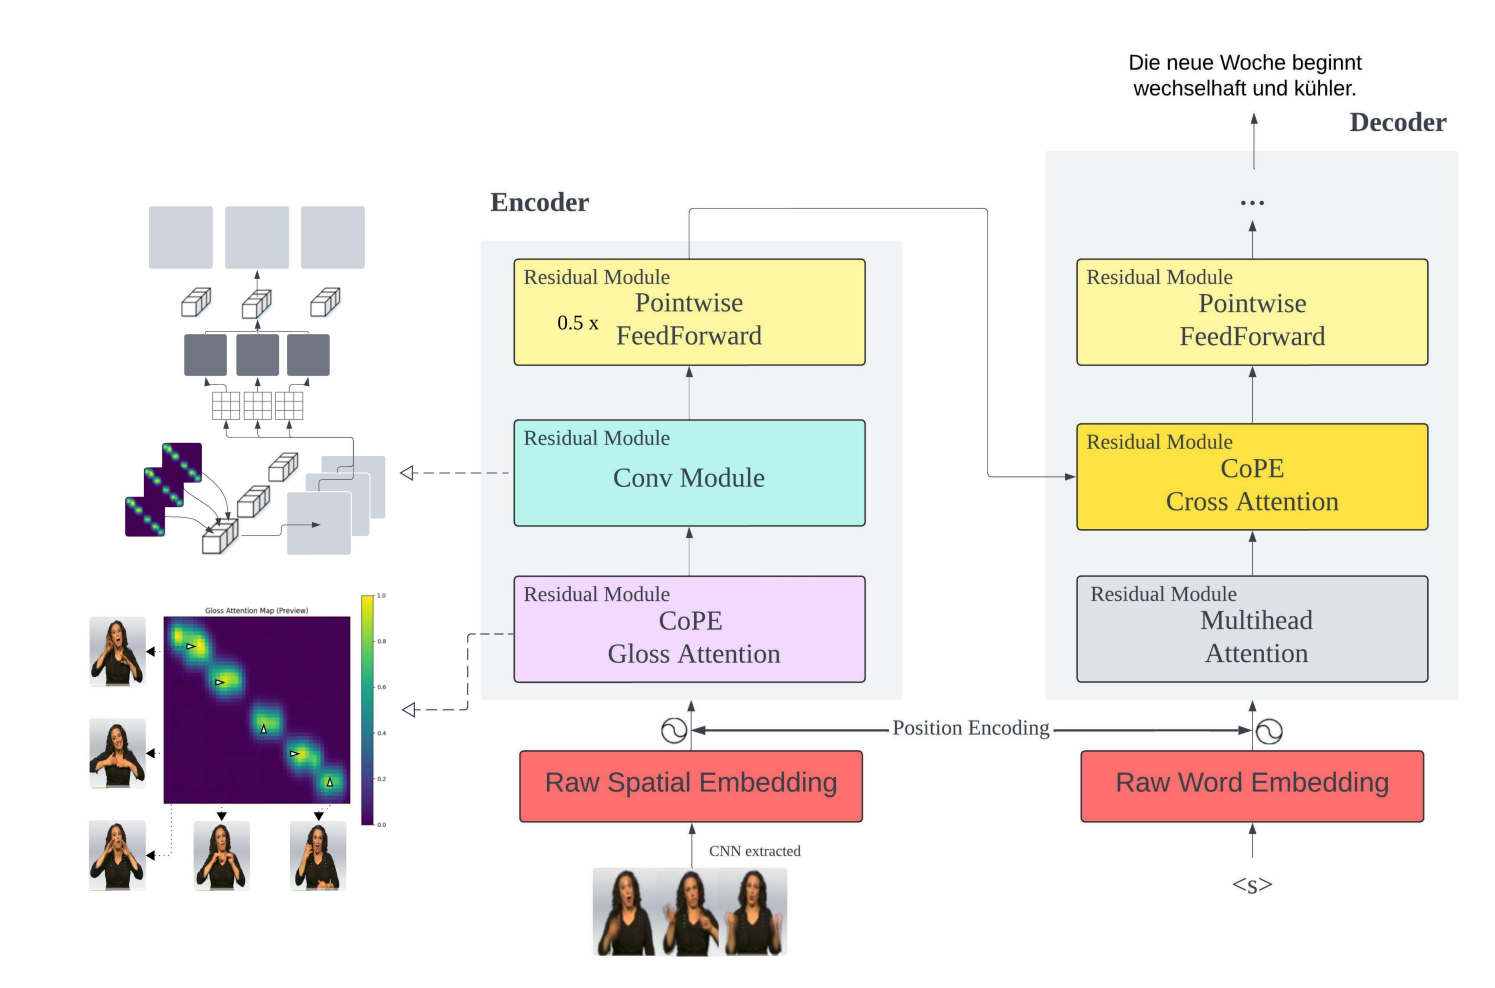
\includegraphics[width=1\textwidth]{../graphics/structuurSignFormer.png}
  \caption{architectuur van Signformer \autocite{eta2024signformer}}  
  \label{fig:signformer}
\end{figure}


\section{Overwegingen bij het Deployen van het Model}
Bij het implementeren van het model voor real-time vertaling van Vlaamse Gebarentaal naar tekst is de keuze van het platform een cruciale factor. 
Twee veelvoorkomende opties zijn een Android-app of een webgebaseerde oplossing. Beide benaderingen hebben hun eigen voordelen en uitdagingen op het gebied van prestaties, toegankelijkheid, gebruikservaring en rekenkracht. 
In deze sectie worden de voor- en nadelen van beide opties besproken, evenals de argumentatie achter de uiteindelijke keuze voor de deploymentstrategie.
\\
\\
Een model kan op twee manieren worden ingezet voor gebruik in een mobiele applicatie: On-device deployment (zie \ref{subsec:on-device}) en Cloud-based deployment (zie \ref{subsec:cloud-based}).
De keuze tussen deze methoden hangt af van factoren zoals real-time prestatie-eisen, energieverbruik, privacy en de technische mogelijkheden van de doelgroep.
\subsection{On-device}
\label{subsec:on-device}
Bij on-device deployment wordt het model lokaal uitgevoerd op het mobiele apparaat van de gebruiker. 
Dit heeft als voordeel dat er geen constante internetverbinding nodig is, wat zorgt voor een lagere latentie en betere privacybescherming. 
Daarnaast kan het model ook offline functioneren, wat cruciaal is voor gebruikers in gebieden met beperkte connectiviteit. 
Echter, on-device inferentie kan intensief zijn op het gebied van rekenkracht en batterijverbruik, zeker bij complexe deep learning-modellen. 
Volgens \textcite{8360327} vereist on-device inferentie vaak optimalisaties zoals modelcompressie of hardwareversnelling met behulp van TensorFlow Lite, ONNX Runtime of Core ML.

\subsection{Cloud-based}
\label{subsec:cloud-based}
Bij cloud-based deployment wordt het model niet op het mobiele apparaat zelf uitgevoerd, maar op een externe server. 
Dit heeft als voordeel dat krachtigere hardware gebruikt kan worden, wat leidt tot snellere inferentie en ondersteuning voor grotere modellen. 
Daarnaast maakt dit het gemakkelijker om updates door te voeren zonder dat de gebruiker iets hoeft te downloaden. 
Het nadeel is echter de afhankelijkheid van een internetverbinding en mogelijke vertragingen door netwerkcommunicatie. 
Bovendien brengt het versturen van gebruikersgegevens naar de cloud privacyrisico’s met zich mee \autocite{8360327}.
Voor toepassingen met strikte real-time vereisten kan dit een beperking vormen.

\subsection{Keuze voor On-device Deployment}
In dit onderzoek is er dan gekozen voor een On-Device oplossing.
De grootste reden hiervoor is de lagere latentie waardoor real-time verwerking mogelijk is.
Omdat het model direct op het apparaat draait, is er geen internetverbinding vereist, wat de applicatie toegankelijker maakt.
\\
\\
Om deze On-Device oplossing te realiseren, wordt de mobiele applicatie ontwikkeld voor het Android-platform. 
Android is een van de meest populaire mobiele besturingssystemen ter wereld, met een breed scala aan apparaten en gebruikers.
De reden dat we niet ook voor iOS ontwikkelen, is dat dit een volledig andere programmeertaal en ontwikkelomgeving met zich meebrengt, wat de ontwikkeltijd aanzienlijk zou verlengen.
\subsection{Keuze van de Programmeertaal}
\label{subsec:keuze-programmeertaal}
Er zijn verschillende programmeertalen en frameworks beschikbaar voor de ontwikkeling van Android-applicaties, elk met hun eigen voordelen:

\begin{itemize}
  \item \textbf{Kotlin}: De officiële taal voor Android-ontwikkeling, biedt moderne syntax, null safety en sterke interoperabiliteit met Java \autocite{google_kotlin}.  
  \item \textbf{Java}: Een veelgebruikte taal voor Android, stabiel en breed ondersteund, maar minder modern dan Kotlin \autocite{java_android}.  
  \item \textbf{React Native (JavaScript)}: Een populaire keuze voor hybride apps, biedt snelle ontwikkeling en brede ondersteuning \autocite{react_native}.  
  \item \textbf{BeeWare (Python)}: Een framework dat het mogelijk maakt om met Python native mobiele apps te ontwikkelen voor meerdere platforms \autocite{beeware}.  
  \item \textbf{C++ (NDK)}: Geschikt voor performance-intensieve toepassingen, zoals deep learning-inferentie op lage niveaus \autocite{android_ndk}.  
\end{itemize}

Kotlin is uiteindelijk gekozen als programmeertaal vanwege de native ondersteuning door Android, de moderne syntax en de sterke interoperabiliteit met Java. 
Java, hoewel stabiel en breed ondersteund, is minder modern en wordt minder aanbevolen door Google. 
React Native werd niet gekozen vanwege de beperkingen in prestaties en toegang tot hardware-specifieke functies. 
BeeWare biedt de mogelijkheid om apps in Python te ontwikkelen, maar Python is minder efficiënt voor mobiele toepassingen en BeeWare is nog in ontwikkeling. 
C++ via het Android NDK biedt uitstekende prestaties voor computationele intensieve toepassingen, maar brengt een hogere ontwikkelcomplexiteit met zich mee, terwijl Kotlin al voldoende prestaties biedt voor de vereisten van dit project.

\subsection{Model voor inferentie op Android}
\label{subsec:model-inferentie-android}

Om een getraind deep learning model, zoals SignFormer, effectief te kunnen inzetten voor real-time inferentie op Android-apparaten, is een essentiële stap de conversie van het model naar een formaat en structuur die compatibel is met de mobiele hardware en softwareomgeving.
Mobiele apparaten hebben veel beperkingen op het gebied van rekenkracht, geheugen en energieverbruik vergeleken met de omgevingen (zoals desktop-GPU's of cloudservers) waarin deze modellen typisch worden getraind.
Daarom is optimalisatie en een specifieke mobiele runtime noodzakelijk.
\\
\\
Historisch gezien was \textbf{PyTorch Mobile} de standaardoplossing binnen het PyTorch-ecosysteem voor het faciliteren van inferentie op mobiele besturingssystemen zoals Android en iOS.
Dit platform stelde ontwikkelaars in staat om modellen getraind in PyTorch te exporteren en deze direct in te bedden in mobiele applicaties, gebruikmakend van een geoptimaliseerde mobiele runtime \autocite{paszke2019pytorch}.
Een cruciaal aspect bij de keuze van een mobiel inferentie-framework, en een reden om in bepaalde gevallen niet te kiezen voor alternatieven zoals TensorFlow Lite \autocite{tensorflow_lite}, is de aanwezigheid van  custom gedefinieerde lagen en/of operaties in het getrainde model.
Hoewel TensorFlow Lite uitstekend presteert met standaardmodelarchitecturen waar bij conversie er standaard ingebouwde operaties zijn \autocite{tflite_ops}, kan de conversie van modellen met custom PyTorch-lagen naar het TensorFlow Lite-formaat leiden tot compatibiliteitsproblemen, dit vereist dan de handmatige implementatie van custom TFLite-operators, of kan zelfs resulteren in verlies van functionaliteit van deze lagen tijdens de conversie.
Door te kiezen voor een oplossing binnen het PyTorch-ecosysteem, zoals PyTorch Mobile (en later ExecuTorch), wordt dit risico enorm beperkt, omdat deze platformen beter zijn uitgerust om een brede reeks van PyTorch-operaties en TorchScript-functionaliteit te ondersteunen, waarbij deze custom lagen en operaties horen.
\\
\\
Recentelijk heeft Meta \textbf{ExecuTorch} geïntroduceerd als een evolutie voor mobiele inferentie vergeleken met PyTorch.
ExecuTorch is een licht, flexibel en modulaire inferentie-engine die specifiek is ontworpen voor een breed spectrum van \textit{edge devices}, waaronder niet alleen smartphones, maar ook wearables, microcontrollers en andere embedded systemen \autocite{executorch2023}.
Het doel van ExecuTorch is om nog verdere optimalisaties en een kleinere voetafdruk te bieden dan traditionele mobiele runtimes.

\subsubsection{Van PyTorch naar mobiele uitvoering: TorchScript en ExecuTorch}
\label{sssec:torchscript-executorch}

Het transitieproces van een getraind PyTorch-model naar een uitvoerbare vorm op mobiele of edge-apparaten begint met de conversie naar \textbf{TorchScript}.
TorchScript fungeert als een intermediaire, seriële representatie van een PyTorch-model dat het computationele graaf en de parameters vastlegt.
Het is ontworpen om los te staan van Python, waardoor het kan worden uitgevoerd in omgevingen waar Python niet beschikbaar is, zoals C++ gebaseerde mobiele runtimes \autocite{pytorch_jit}.
Er zijn twee primaire methoden om TorchScript te genereren vanuit een PyTorch-model:
\begin{itemize}
    \item \textit{Scripting (\texttt{torch.jit.script})}: Deze methode analyseert de Python-broncode van het model en compileert deze naar TorchScript.
Dit is vooral krachtig voor modellen die control flow structuren bevatten (zoals if/else-voorwaarden of lussen) die afhankelijk zijn van de inputdata.
    \item \textit{Tracing (\texttt{torch.jit.trace})}: Bij tracing wordt het model uitgevoerd met voorbeeld data, waarbij de sequentie van uitgevoerde operaties wordt geregistreerd en vastgelegd in het TorchScript-formaat.
Deze methode is eenvoudiger toe te passen, maar kan beperkingen hebben bij input-afhankelijke control flow.
\end{itemize}
De keuze tussen scripting en tracing hangt af van de specifieke architectuur en implementatie van het model.
Voor custom lagen is het cruciaal dat hun implementatie compatibel is met het TorchScript-conversieproces, wat bij scripting meer controle vereist over de Python-code en bij tracing afhangt van hoe de custom operaties intern worden afgehandeld.
\\
\\
Voor conventionele mobiele Android-applicaties kan dit TorchScript-model direct worden geladen en uitgevoerd met behulp van de \textit{PyTorch Mobile runtime}.
Dit bied een relatief eenvoudige weg voor de integratie van getrainde PyTorch-modellen.
ExecuTorch bouwt voort op TorchScript, maar biedt een meer precieze controle over het deploymentproces. 
Het ondersteunt eveneens TorchScript-modellen als invoer. 
Dit framework is speciaal ontworpen voor veeleisende scenario's op edge-apparaten, waarbij de focus ligt op maximale reductie van de binaire grootte, minimale latentie en diepe integratie met C++-gebaseerde embedded systemen. 
ExecuTorch vertegenwoordigt zo een verschuiving naar meer controle over de implementatie van modellen op diverse edge-hardware \autocite{executorch2023}. 
ExecuTorch voegt een fase toe voor verdere graaf transformatie en optimalisatie, gericht op specifieke hardwarebackends en resourcebeperkingen.

\subsubsection{Modeloptimalisatie via kwantisatie}
\label{sssec:model-optimalisatie-kwantisatie}

Ongeacht het gekozen inferentieplatform (PyTorch Mobile of ExecuTorch), is \textbf{kwantisatie} een cruciale aanvullende optimalisatiestap die niet automatisch wordt uitgevoerd.
Kwantisatie is een techniek waarbij de numerieke precisie van de modelparameters (gewichten, biases) en soms ook de intermediaire activaties wordt gereduceerd, doorgaans van 32-bit floating-point getallen naar lagere-precisie formaten zoals 8-bit integers \autocite{quantization_survey}.
De primaire doelen van kwantisatie zijn het significant verkleinen van de modelgrootte en het versnellen van de inferentie, aangezien berekeningen met lagere-precisie getallen sneller en energiezuiniger kunnen zijn op mobiele en embedded processors.
Kwantisatie introduceert echter ruis en kan leiden tot een reductie in modelnauwkeurigheid, wat zorgvuldige afweging en validatie vereist.

Er zijn twee voorname kwantisatiemethoden die relevant zijn voor mobiele deployment:
\begin{itemize}
    \item \textbf{Post-training kwantisatie (PTQ)}: Bij PTQ wordt kwantisatie toegepast op een model nadat het volledig is getraind.
Dit is over het algemeen de eenvoudigste methode omdat het geen aanpassingen aan het trainingsproces vereist.
Zowel PyTorch Mobile als ExecuTorch bieden tools en workflows voor PTQ \autocite{krishnamoorthi2018quantization}.
Verschillende varianten bestaan, zoals Dynamic Quantization (waarbij activaties dynamisch worden gekwantiseerd tijdens inferentie) en Static Quantization (waarbij de kwantisatieparameters voor activaties vooraf worden bepaald met behulp van een representatieve dataset).
    \item \textbf{Kwantisatie-bewuste training (Quantization-Aware Training - QAT)}: QAT simuleert het effect van kwantisatie tijdens het trainingsproces zelf.
Dit stelt het model in staat om zich aan te passen aan de kwantisatieruis, wat vaak resulteert in een hogere nauwkeurigheid van het gekwantiseerde model vergeleken met PTQ, dit is ten koste van een complexer trainingsproces.
Ook voor QAT bieden zowel PyTorch Mobile als ExecuTorch ondersteuning.
\end{itemize}
Beide platformen bieden ondersteuning voor deze optimalisatietechnieken, waarbij ExecuTorch, gezien zijn focus op edge devices, vaak meer nadruk legt op de integratie met hardware-acceleratoren en de optimalisatie van de runtime voor kwantisatie op beperkte hardware.

\subsubsection{Toepassing in Android-omgevingen}
\label{sssec:toepassing-android}

Voor de ontwikkeling van mobiele Android-applicaties die gebruik maken van PyTorch-modellen voor inferentie, blijft het pad van TorchScript en de \textit{PyTorch Mobile runtime} de meest directe en breed ondersteunde aanpak.
Het geoptimaliseerde TorchScript-model (vaak in een specifiek mobiel formaat zoals `.ptl`) wordt als resource opgenomen in het Android-applicatiepakket (APK).
De PyTorch Android API wordt vervolgens gebruikt om dit model tijdens runtime te laden en inferentie uit te voeren, waarbij de inputdata (bijvoorbeeld verwerkte cameraframes) als tensors aan het model worden aangeboden.
\\
\\
ExecuTorch is met name relevant voor meer geavanceerde of resource-beperkte scenario's binnen het Android-ecosysteem, of voor integratie met native (C++) codebases waar minimale overhead cruciaal is.
Hoewel ExecuTorch op Android kan worden ingezet, is de typische workflow meer gericht op cross-compilatie voor specifieke doelplatforms en diepere integratie met de onderliggende C++-runtimeomgevingen, in tegenstelling tot de hogere-niveau Java/Kotlin API die beschikbaar is via PyTorch Mobile.
De keuze tussen deze twee benaderingen voor een Android-applicatie hangt af van factoren zoals de prestatie-eisen, de gewenste binaire grootte, de complexiteit van het model, de noodzaak voor custom operator-integratie en de mate van controle die nodig is over de inferentie-pipeline en hardware-interactie.
Voor de meeste standaardgebruiksscenario's in een mobiele app biedt PyTorch Mobile een robuuste en toegankelijke oplossing.
